\section{mo\-HCMove\-Loop\-Expl$<$ M $>$ Class Template Reference}
\label{classmo_h_c_move_loop_expl}\index{moHCMoveLoopExpl@{moHCMoveLoopExpl}}
Iterative explorer used by a {\bf mo\-HC}{\rm (p.\,\pageref{classmo_h_c})}.  


{\tt \#include $<$mo\-HCMove\-Loop\-Expl.h$>$}

Inheritance diagram for mo\-HCMove\-Loop\-Expl$<$ M $>$::\begin{figure}[H]
\begin{center}
\leavevmode
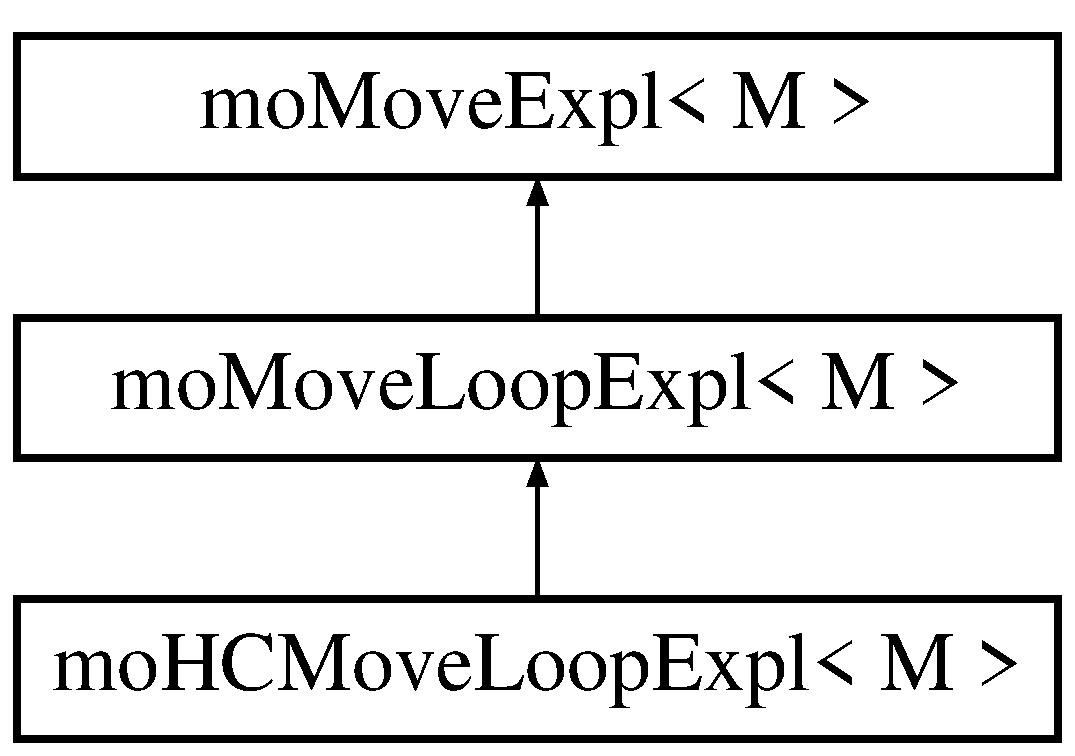
\includegraphics[height=3cm]{classmo_h_c_move_loop_expl}
\end{center}
\end{figure}
\subsection*{Public Member Functions}
\begin{CompactItemize}
\item 
{\bf mo\-HCMove\-Loop\-Expl} ({\bf mo\-Move\-Init}$<$ M $>$ \&\_\-\_\-move\_\-init, {\bf mo\-Next\-Move}$<$ M $>$ \&\_\-\_\-next\_\-move, {\bf mo\-Move\-Incr\-Eval}$<$ M $>$ \&\_\-\_\-incr\_\-eval, {\bf mo\-Move\-Select}$<$ M $>$ \&\_\-\_\-move\_\-select)
\begin{CompactList}\small\item\em Constructor. \item\end{CompactList}\item 
void {\bf operator()} (const {\bf EOT} \&\_\-\_\-old\_\-sol, {\bf EOT} \&\_\-\_\-new\_\-sol)
\begin{CompactList}\small\item\em Procedure which launches the explorer. \item\end{CompactList}\end{CompactItemize}
\subsection*{Private Types}
\begin{CompactItemize}
\item 
typedef M::EOType {\bf EOT}\label{classmo_h_c_move_loop_expl_077befd4106c201eafd3ea22bcea2fe9}

\begin{CompactList}\small\item\em Alias for the type. \item\end{CompactList}\item 
typedef M::EOType::Fitness {\bf Fitness}\label{classmo_h_c_move_loop_expl_f24871224316d5549b9013a2d27ab465}

\begin{CompactList}\small\item\em Alias for the fitness. \item\end{CompactList}\end{CompactItemize}
\subsection*{Private Attributes}
\begin{CompactItemize}
\item 
{\bf mo\-Move\-Init}$<$ M $>$ \& {\bf move\_\-init}\label{classmo_h_c_move_loop_expl_6776fc51331c1b452d026b92448b4ffc}

\begin{CompactList}\small\item\em Move initialiser. \item\end{CompactList}\item 
{\bf mo\-Next\-Move}$<$ M $>$ \& {\bf next\_\-move}\label{classmo_h_c_move_loop_expl_f716c5271e0eba9275c585dc52768443}

\begin{CompactList}\small\item\em Neighborhood explorer. \item\end{CompactList}\item 
{\bf mo\-Move\-Incr\-Eval}$<$ M $>$ \& {\bf incr\_\-eval}\label{classmo_h_c_move_loop_expl_84a8fccba05ab30414281469bc8ee779}

\begin{CompactList}\small\item\em (generally) Efficient evaluation. \item\end{CompactList}\item 
{\bf mo\-Move\-Select}$<$ M $>$ \& {\bf move\_\-select}\label{classmo_h_c_move_loop_expl_13bcd1322b2b97fd665be2f60c532fbb}

\begin{CompactList}\small\item\em Move selector. \item\end{CompactList}\end{CompactItemize}


\subsection{Detailed Description}
\subsubsection*{template$<$class M$>$ class mo\-HCMove\-Loop\-Expl$<$ M $>$}

Iterative explorer used by a {\bf mo\-HC}{\rm (p.\,\pageref{classmo_h_c})}. 



Definition at line 23 of file mo\-HCMove\-Loop\-Expl.h.

\subsection{Constructor \& Destructor Documentation}
\index{moHCMoveLoopExpl@{mo\-HCMove\-Loop\-Expl}!moHCMoveLoopExpl@{moHCMoveLoopExpl}}
\index{moHCMoveLoopExpl@{moHCMoveLoopExpl}!moHCMoveLoopExpl@{mo\-HCMove\-Loop\-Expl}}
\subsubsection{\setlength{\rightskip}{0pt plus 5cm}template$<$class M$>$ {\bf mo\-HCMove\-Loop\-Expl}$<$ M $>$::{\bf mo\-HCMove\-Loop\-Expl} ({\bf mo\-Move\-Init}$<$ M $>$ \& {\em \_\-\_\-move\_\-init}, {\bf mo\-Next\-Move}$<$ M $>$ \& {\em \_\-\_\-next\_\-move}, {\bf mo\-Move\-Incr\-Eval}$<$ M $>$ \& {\em \_\-\_\-incr\_\-eval}, {\bf mo\-Move\-Select}$<$ M $>$ \& {\em \_\-\_\-move\_\-select})\hspace{0.3cm}{\tt  [inline]}}\label{classmo_h_c_move_loop_expl_11410d648d79746253e9dc249c4ec7b5}


Constructor. 

All the boxes have to be specified.

\begin{Desc}
\item[Parameters:]
\begin{description}
\item[{\em \_\-\_\-move\_\-init}]the move initialiser. \item[{\em \_\-\_\-next\_\-move}]the neighborhood explorer. \item[{\em \_\-\_\-incr\_\-eval}](generally) efficient evaluation function. \item[{\em \_\-\_\-move\_\-select}]the move selector. \end{description}
\end{Desc}


Definition at line 43 of file mo\-HCMove\-Loop\-Expl.h.

\subsection{Member Function Documentation}
\index{moHCMoveLoopExpl@{mo\-HCMove\-Loop\-Expl}!operator()@{operator()}}
\index{operator()@{operator()}!moHCMoveLoopExpl@{mo\-HCMove\-Loop\-Expl}}
\subsubsection{\setlength{\rightskip}{0pt plus 5cm}template$<$class M$>$ void {\bf mo\-HCMove\-Loop\-Expl}$<$ M $>$::operator() (const {\bf EOT} \& {\em \_\-\_\-old\_\-sol}, {\bf EOT} \& {\em \_\-\_\-new\_\-sol})\hspace{0.3cm}{\tt  [inline]}}\label{classmo_h_c_move_loop_expl_f48d5379caac7f6a165e9fe8840e6ccb}


Procedure which launches the explorer. 

The exploration starts from an old solution and provides a new solution.

\begin{Desc}
\item[Parameters:]
\begin{description}
\item[{\em \_\-\_\-old\_\-sol}]the current solution. \item[{\em \_\-\_\-new\_\-sol}]the new\_\-sol (result of the procedure). \end{description}
\end{Desc}


Definition at line 59 of file mo\-HCMove\-Loop\-Expl.h.

References mo\-HCMove\-Loop\-Expl$<$ M $>$::incr\_\-eval, mo\-HCMove\-Loop\-Expl$<$ M $>$::move\_\-init, mo\-HCMove\-Loop\-Expl$<$ M $>$::move\_\-select, and mo\-HCMove\-Loop\-Expl$<$ M $>$::next\_\-move.

The documentation for this class was generated from the following file:\begin{CompactItemize}
\item 
mo\-HCMove\-Loop\-Expl.h\end{CompactItemize}
